%%%%%%%%%%%%%%%%%%%%%%%%%%%%%%%%%%%%%%%%%%%%%%%%%%%%
\chapter{Inductance Characterization}\label{Appendix: AA}
\section{Inductance Estimation Table}



\section{Equivalent coil impedance} \label{AppendixSection: impedance}






%%%%%%%%%%%%%%%%%%%%%%%%%%%%%%%%%%%%%%%%%%%%%%%%%%%%
%%%%%%%%%%%%%%%%%%%%%%%%%%%%%%%%%%%%%%%%%%%%%%%%%%%%
%%%%%%%%%%%%%%%%%%%%%%%%%%%%%%%%%%%%%%%%%%%%%%%%%%%%
%%%%%%%%%%%%%%%%%%%%%%%%%%%%%%%%%%%%%%%%%%%%%%%%%%%%
\chapter{Model equations} \label{Appendix: A}
\section{Secondary capacitor in series} \label{sec:secondaryS}



\section{Secondary capacitor in parallel}\label{sec:secondaryP}

The same steps as above are followed for obtaining the impedances $Z_2$ and $Z_R$ when the secondary capacitor is placed in parallel: 


%%%%%%%%%%%%%%%%%%%%%%%%%%%%%%%%%%%%%%%%%%%%%%%%%%%%
%%%%%%%%%%%%%%%%%%%%%%%%%%%%%%%%%%%%%%%%%%%%%%%%%%%%
%%%%%%%%%%%%%%%%%%%%%%%%%%%%%%%%%%%%%%%%%%%%%%%%%%%%







%%%%%%%%%%%%%%%%%%%%%%%%%%%%%%%%%%%%%%%%%%%%%%%%%%%%
\chapter{Coils Experimental Results}
\section{Inductance and Resistance}\label{sec:RL}




\section{Quality Factor}








%%%%%%%%%%%%%%%%%%%%%%%%%%%%%%%%%%%%%%%%%%%%%%%%%%%%
%%%%%%%%%%%%%%%%%%%%%%%%%%%%%%%%%%%%%%%%%%%%%%%%%%%%
\chapter{Circuit Schematics}

\section{Voltage Regulator}\label{Appendix: DC-DC}

% \begin{figure}[htb]
% 	\begin{center}
% 		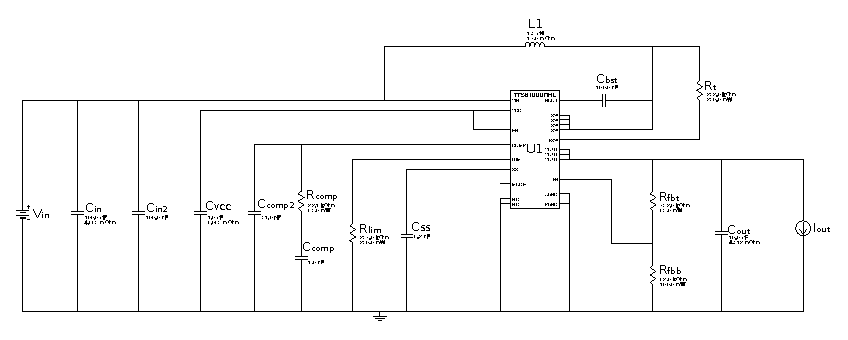
\includegraphics[width=1.05\textwidth]{./images/TPS61088}
% 	\caption{TPS61088 design circuit}
% 	\end{center}
% \end{figure}

\begin{figure}[htb]
	\begin{center}
		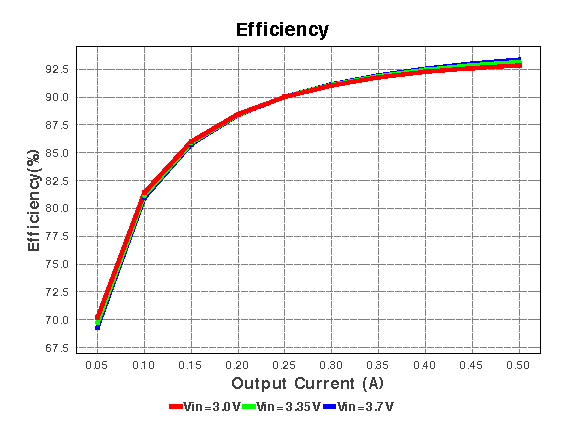
\includegraphics[width=0.8\textwidth]{./images/Efficiency_TPS61088}
	\caption{Efficiency w.r.t. output current}
	\end{center}
\end{figure}

\section{Power Driver}\label{Appendix: powerDriver}
% \begin{figure}[H]
% 	\begin{center}
% 		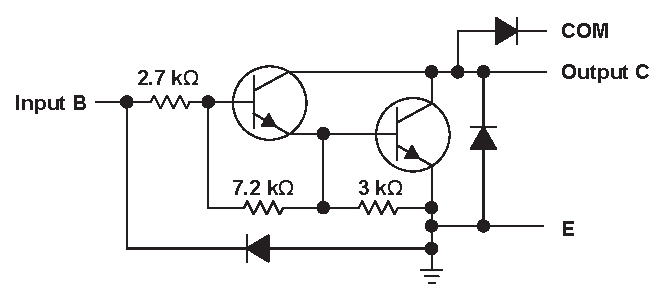
\includegraphics[width=0.8\textwidth]{./images/ULN2803A}
% 	\caption{Functional block diagram of the ULN2803A}
% 	\end{center}
% \end{figure}

\begin{figure}[H]
\centering
\begin{subfigmatrix}{2} 
\hspace*{\fill}%
\subfigure[Functional block diagram] 
	{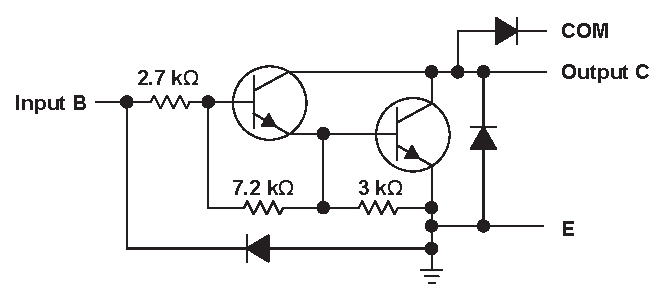
\includegraphics[width=3.0in]{./images/ULN2803A}}\hfill
\subfigure[Top view]
	{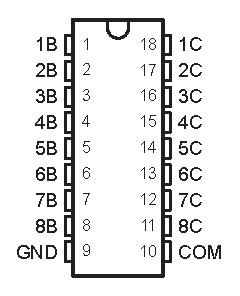
\includegraphics[width=1.0in]{./images/ulnpins}}
\hspace*{\fill}%
\end{subfigmatrix}
\caption{ULN2803 Darlington driver}
\end{figure}


\section{Transmitter}

\begin{figure}[H]
\begin{center}
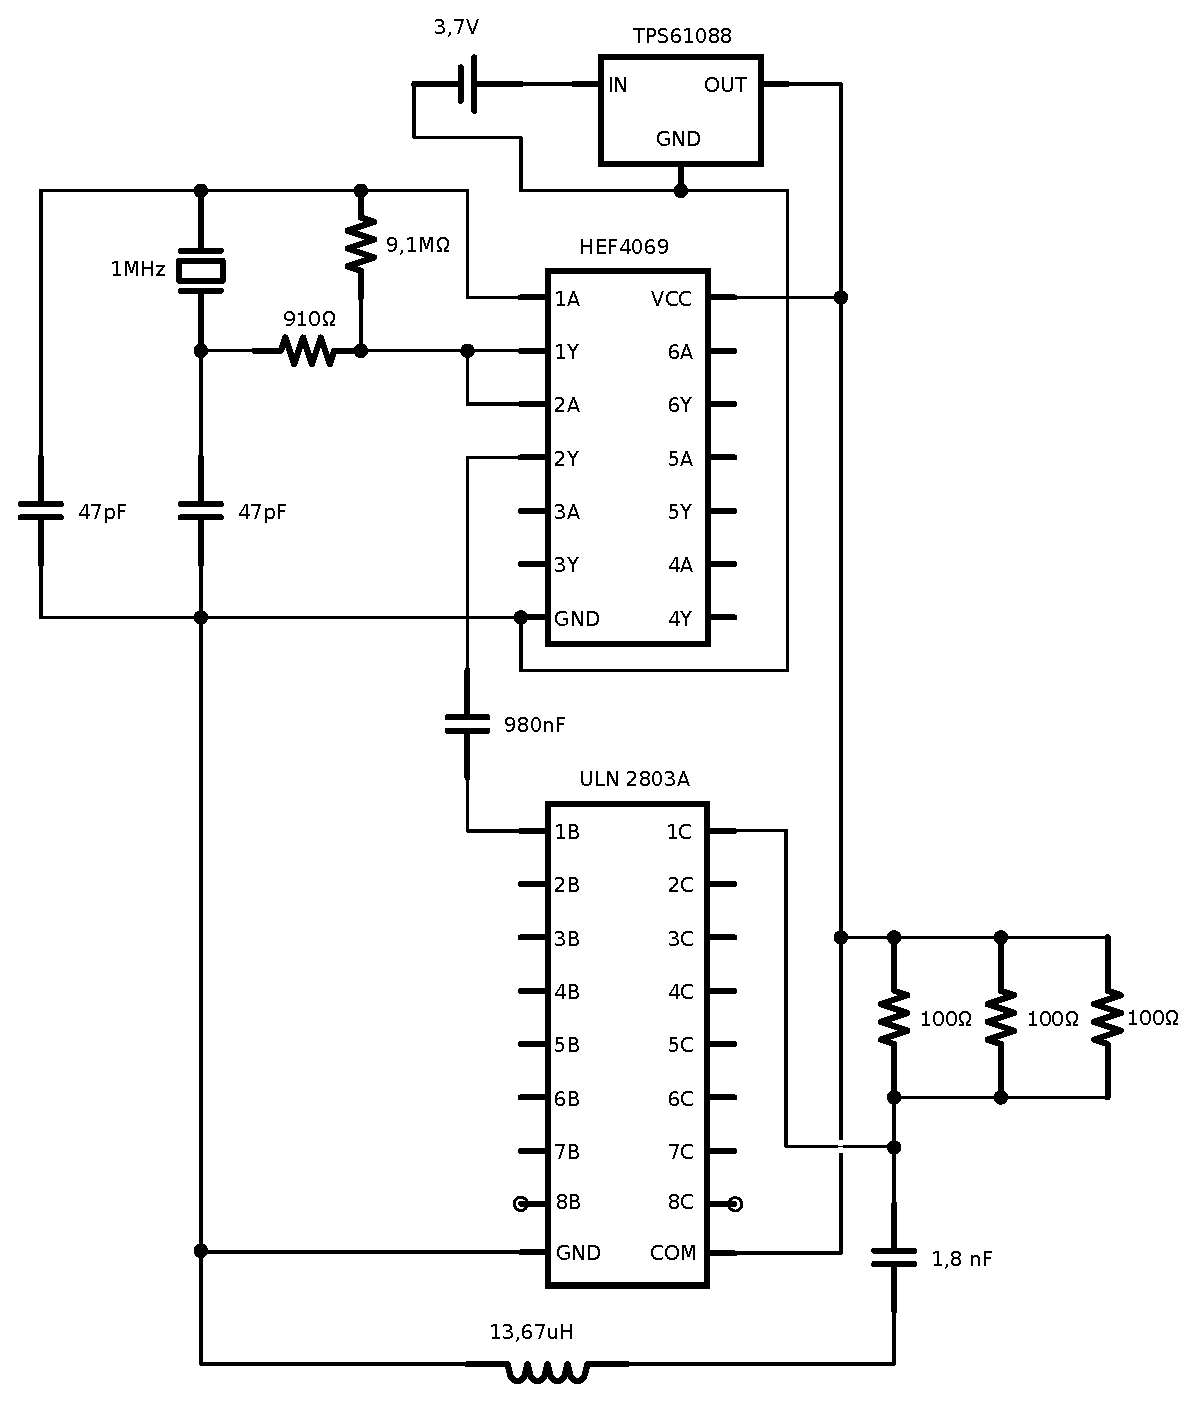
\includegraphics[width=1\textwidth]{./images/circuitv5}
\caption{Transmitter circuit schematic}
% \label{F:contourLines}
\end{center}
\end{figure}

\section{Receiver}
\begin{figure}[H]
\begin{center}
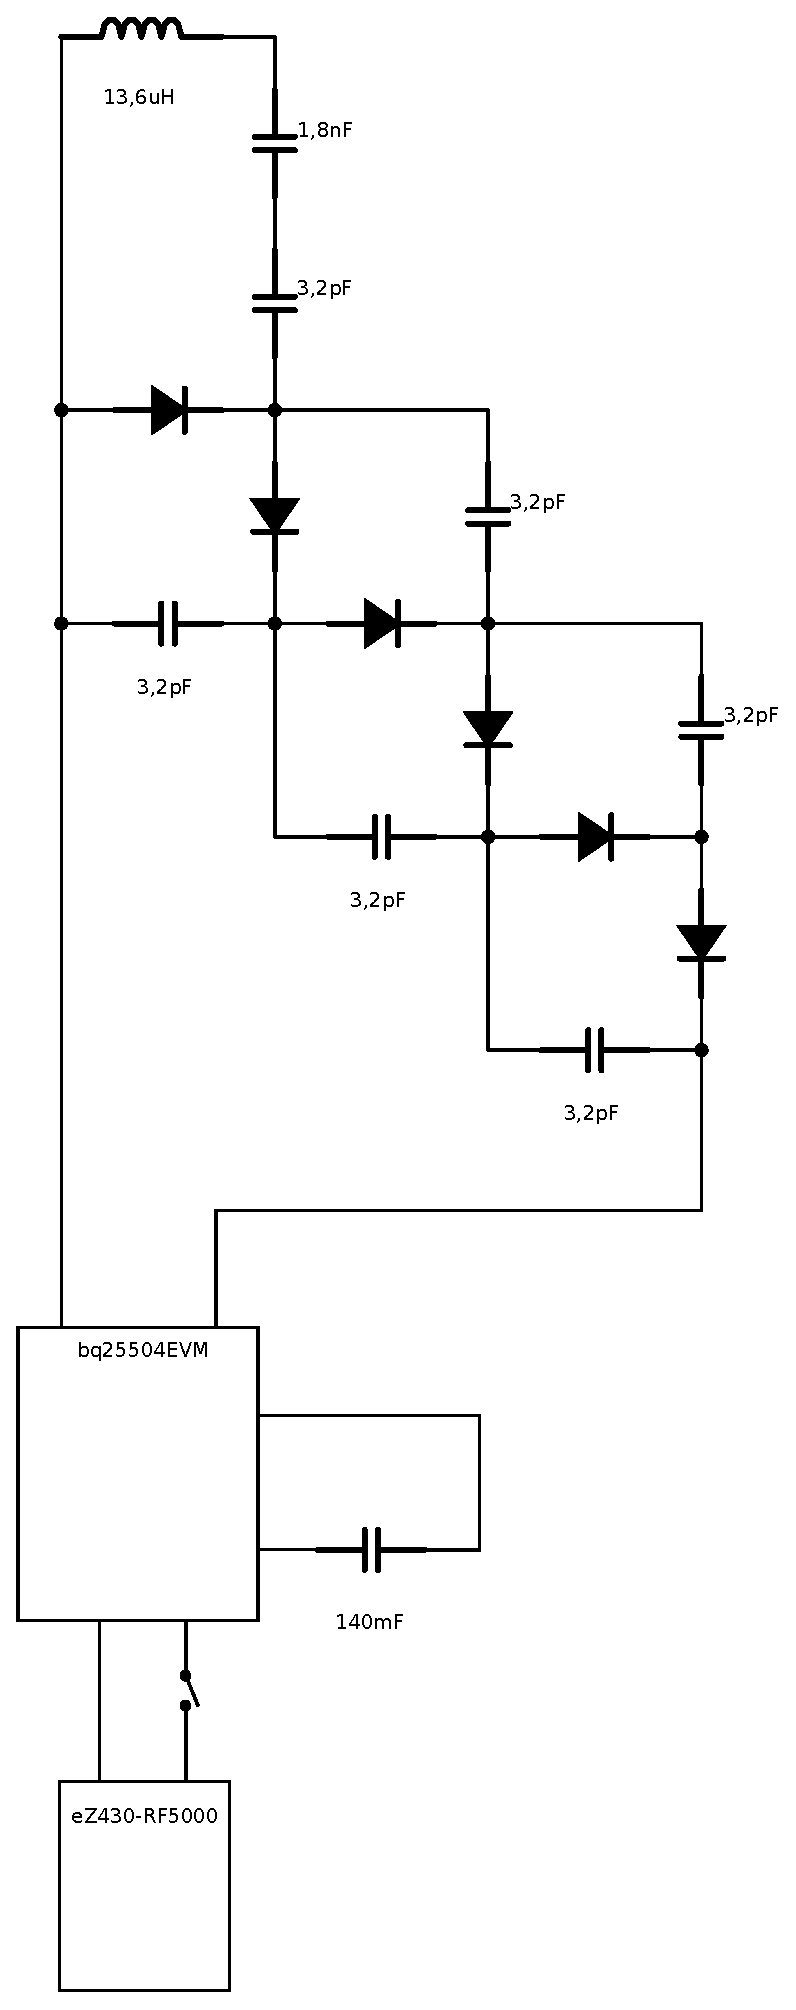
\includegraphics[width=0.55\textwidth]{./images/ReceiverSchematic}
\caption{Receiver circuit schematic}
% \label{F:contourLines}
\end{center}
\end{figure}

